\documentclass[letterpaper,12pt,fleqn]{article}
\usepackage{matharticle}
\usepackage{tikz}
\pagestyle{plain}
\begin{document}

\begin{center}
\Large Math-19 Exam \#1
\end{center}

\vspace{0.5in}

Name: \rule{4in}{1pt}

\vspace{0.5in}

This exam is closed book and notes. You may use a calculator; however, no cell
phones or tablets are allowed. Show all work; there is no credit for guessed
answers. All values should be exact unless you are specifically asked for an
approximate value answer.

\vspace{0.5in}

\newcommand{\fillin}{\rule{2in}{1pt}}
\newcommand{\sfillin}{\rule{0.5in}{1pt}}

\begin{enumerate}
\item (20 points) The following questions are related to the classifications of
the real numbers:
\begin{enumerate}
\item Identify each subset of the real numbers and give an example of an
element from each set.

\begin{tabular}{ccc}
subset & identify & example \\
\\
$\N$ & \fillin & \sfillin \\
\\
$\Z$ & \fillin & \sfillin \\
\\
$\Q$ & \fillin & \sfillin \\
\\
$\R-\Q$ & \fillin & \sfillin \\
\\
$\R$ & \fillin & \sfillin \\
\end{tabular}

\vspace{0.5in}

\item Convert the number $2.1\overline{35}$ to rational form.
\vspace{3in}
\end{enumerate}

\newpage

\item (10 points) Identify each of the following formulas:

\vspace{0.25in}

\begin{tabular}{cc}
$a^2+b^2=c^2$ & \fillin \\
\\
$d=[(x_1-x_2)^2+(y_1-y_2)^2]^{1/2}$ & \fillin \\
\\
$\left(\frac{x_1+x_2}{2},\frac{y_1+y_2}{2}\right)$ & \fillin \\
\\
$m=\frac{y_1-y_2}{x_1-x_2}$ & \fillin \\
\\
$y-y_1=m(x-x_1)$ & \fillin \\
\\
$y=mx+b$ & \fillin \\
\\
$Ax+By+C=0$ & \fillin \\
\\
$m_1=m_2$ & \fillin \\
\\
$m_1m_2=-1$ & \fillin \\
\\
$(x-h)^2+(y-k)^2=r^2$ & \fillin \\
\\
$x^2+Ax+y^2+By+C=0$ & \fillin \\
\\
$x=\frac{-b\pm\sqrt{b^2-4ac}}{2a}$ & \fillin \\
\end{tabular}

\newpage

\item (20 points) You have two dogs: Fido and Fluffy. Each dog is tied to its
own stake in your backyard by a leash. Fido's stake and leash allow him to roam
around an area defined by:
\[(x-2)^2+(y-1)^2=9\]
Fluffy's stake and leash allow her to roam around an area defined by:
\[x^2+y^2-10x-8y+37=0\]
\begin{enumerate}
\item What are the coordinates of Fido's stake and the length of his leash?

\vspace{0.5in}

\item What are the coordinates of Fluffy's stake and the length of her leash?

\vspace{1.5in}

\item What is the equation of the line between the two stakes, in
slope-intercept form?

\vspace{1.5in}

\item It is mating season. Fido and Fluffy and not fixed, but you do not want
them to mate. To be safe, you decide to erect a straight wall that is
perpendicular to the line joining the two stakes and going through the midpoint
of that line. What is the equation of the wall, in slope-intercept form?
\end{enumerate}

\newpage

\item (10 points) Identify each of the following standard functions:

\vspace{0.25in}

\begin{tabular}{cc}
\begin{tikzpicture}
\draw [<->] (-2,0) -- (2,0);
\draw [<->] (0,-2) -- (0,2);
\draw [domain=-2:2] plot (\x,{\x});
\node at (-1,-3) {$y=$};
\end{tikzpicture} \hspace{1in} &
\begin{tikzpicture}
\draw [<->] (-2,0) -- (2,0);
\draw [<->] (0,-2) -- (0,2);
\draw [domain=-2:2] plot (\x,{abs(\x)});
\node at (-1,-3) {$y=$};
\end{tikzpicture} \\
\end{tabular}

\begin{tabular}{cc}
\begin{tikzpicture}
\draw [<->] (-2,0) -- (2,0);
\draw [<->] (0,-2) -- (0,2);
\draw [domain=0:2] plot (\x,{sqrt(\x)});
\node at (-1,-3) {$y=$};
\end{tikzpicture} \hspace{1in} &
\begin{tikzpicture}
\draw [<->] (-2,0) -- (2,0);
\draw [<->] (0,-2) -- (0,2);
\draw [domain=0:2] plot (\x,{(\x)^(1/3)});
\draw [domain=-2:0] plot (\x,{-(-\x)^(1/3)});
\node at (-1,-3) {$y=$};
\end{tikzpicture} \\
\end{tabular}

\begin{tabular}{cc}
\begin{tikzpicture}
\draw [<->] (-2,0) -- (2,0);
\draw [<->] (0,-2) -- (0,2);
\draw [domain=-1.4:1.4] plot (\x,{(\x)^2});
\node at (-1,-3) {$y=$};
\end{tikzpicture} \hspace{1in} &
\begin{tikzpicture}
\draw [<->] (-2,0) -- (2,0);
\draw [<->] (0,-2) -- (0,2);
\draw [domain=-1.25:1.25] plot (\x,{(\x)^3});
\node at (-1,-3) {$y=$};
\end{tikzpicture} \\
\end{tabular}

\newpage

\item (20 points) Consider the function:
\[f(x)=-(x-1)^2+4\]
\begin{enumerate}
\item Provide a list of transformations, starting from a basic function, for the
function in the order that they are applied (i.e., inside-out).
\begin{enumerate}
\item
\item
\item
\item
\end{enumerate}

\item Determine any x-intercepts.

\vspace{2in}

\item Determine any y-intercepts.

\vspace{1in}

\item Sketch the function. Be sure to label all key points!

\vspace{3in}
\end{enumerate}

\newpage

\item (20 points) You are a product manager at an electronics firm in charge of
a proposed new line of 25-inch monitors (i.e., the length of the diagonal
across the screen is 25 inches):

\bigskip

\begin{figure}[h]
\setlength{\leftskip}{1in}
\begin{tikzpicture}
\draw (0,0) rectangle (5,3);
\draw [dashed] (0,0) -- (5,3);
\node at (2.5,2.0) {25''};
\node [above] at (2.5,0) {$\ell$};
\node [right] at (0,1.5) {$w$};
\end{tikzpicture}
\end{figure}

You realize that the most appealing ratio for the dimensions of the screen
would follow the golden ratio:
\[\frac{\ell}{w}=\frac{1+\sqrt{5}}{2}\approx1.6=\frac{8}{5}\]

\vspace{0.25in}

\begin{enumerate}
\item Using the estimate of $8/5$, determine the dimensions ($\ell\times w$)
for the new monitor. Round each dimension to two decimal places.

\newpage

\item There needs to be an equal amount of casing around the edges of the
screen and the packaging department would like the monitor to have a total
area of 400 square inches.

\begin{figure}[h]
\setlength{\leftskip}{1in}
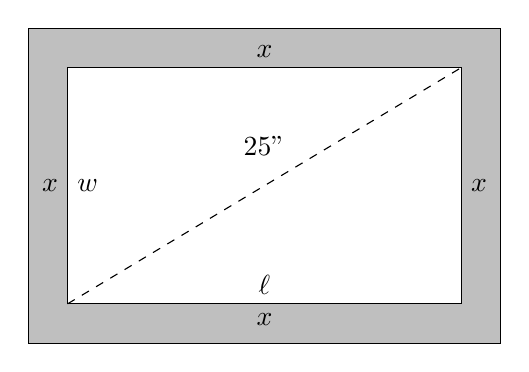
\begin{tikzpicture}
\draw [fill=lightgray] (-0.5,-0.5) rectangle (5.5,3.5);
\draw [fill=white] (0,0) rectangle (5,3);
\draw [dashed] (0,0) -- (5,3);
\node at (2.5,2.0) {25''};
\node [above] at (2.5,0) {$\ell$};
\node [right] at (0,1.5) {$w$};
\node [above] at (2.5,3) {$x$};
\node [below] at (2.5,0) {$x$};
\node [left] at (0,1.5) {$x$};
\node [right] at (5,1.5) {$x$};
\end{tikzpicture}
\end{figure}

Determine the width of the casing ($x$) around the screen. Round your answer to
two decimal places.
\end{enumerate}

\end{enumerate}

\end{document}
